\section{Karte und Gelände}


\begin{frame}[c]{Karte und Gelände}
    \Large
    \pause
    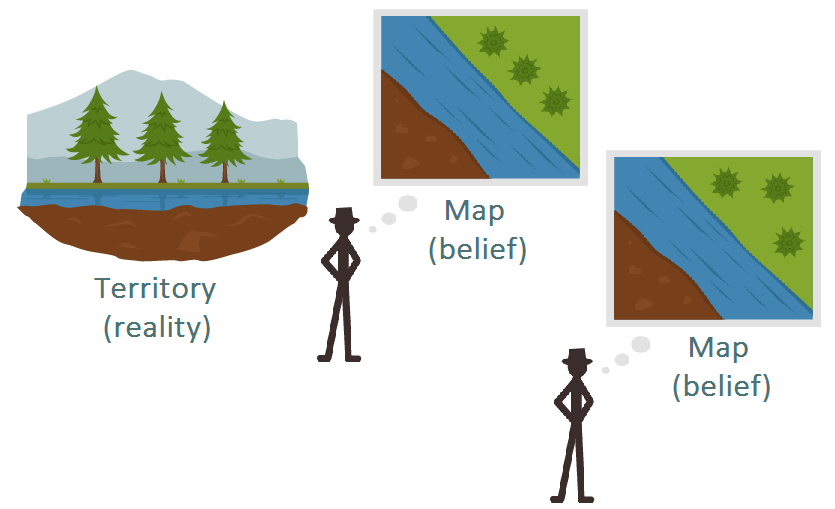
\includegraphics[height=0.85\textheight]{map_territory}
\end{frame}


\begin{frame}[c]{Falsche Erklärungen}
    \only<1>{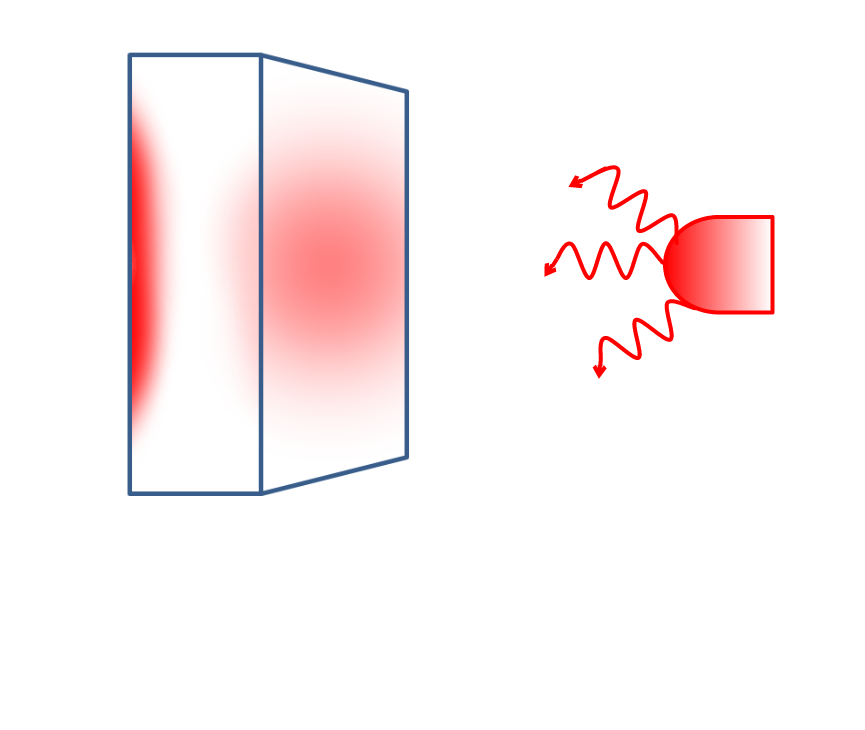
\includegraphics[height=0.95\textheight]{fake_expl_0}}
    \only<2>{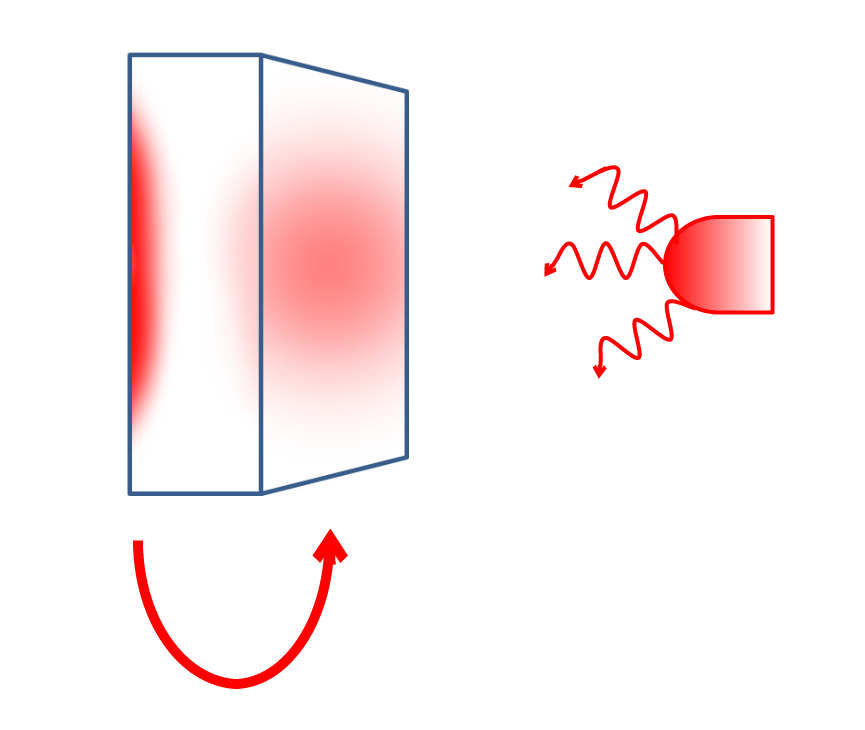
\includegraphics[height=0.95\textheight]{fake_expl_1}}
\end{frame}


\begin{frame}[c]{Eigenschaften eines Rationalisten}
    \Large
    \pause
    Von Fiktion verwirrter zu sein als von der Realität.
    \newline
    \newline
    \pause
    Wenn man jedes Ergebnis gleich gut erklären kann, hat man es nicht verstanden.
\end{frame}



